%%%%%%%%%%%%%%%%%%%%%%%%%%%%%%%%%%%%%%%%%%%%%%%%%%%%%%%%%%%%%%%%%%%%%%%%%%%%%%%
% DCC 2027 submission draft
% Derived from drafts/ieee_tcsvt_submission_20260904/main.tex and the figures
% figures embedded in drafts/RBM_merger_aware_中文_Fig1更新版.docx.
%%%%%%%%%%%%%%%%%%%%%%%%%%%%%%%%%%%%%%%%%%%%%%%%%%%%%%%%%%%%%%%%%%%%%%%%%%%%%%%
\documentclass[smallabstract,smallcaptions]{dccpaper}

\usepackage{amsmath,amssymb}
\usepackage{booktabs}
\usepackage{graphicx}
\usepackage{multirow}
\usepackage{placeins}
\usepackage{url}
\usepackage{xspace}
\usepackage{IEEEtrantools}
\usepackage[hidelinks]{hyperref}
\hypersetup{
  pdftitle={Rank Before You Merge: Training-Free Machine-Centric Visual Token Compression for Efficient Vision-Language Model Inference},
  pdfauthor={Zhengxing Yan},
  pdfsubject={DCC 2027 submission draft},
  pdfkeywords={visual token compression, vision-language models, training-free inference, native merger}
}

\newlength{\figurewidth}
\newlength{\smallfigurewidth}
\setlength{\smallfigurewidth}{2.75in}
\setlength{\figurewidth}{6in}
\newcommand{\pp}{\,pp\xspace}

\begin{document}
\bstctlcite{dccBSTcontrol}

\title{\large\textbf{Rank Before You Merge: Training-Free Machine-Centric
Visual Token Compression for Efficient Vision-Language Model Inference}}

\author{\shortstack{Zhengxing Yan\\[0.5em]
{\small Affiliation to be confirmed}\\
{\small Country and email to be confirmed}}}

\maketitle
\thispagestyle{empty}

\begin{abstract}
Native spatial mergers already compress visual patches before a
vision-language model (VLM) reaches its language model, yet most token
selectors rank the merger outputs. We call compression \emph{machine-centric}
when its units, budget, and interface follow the deployed model's native
computation graph. Rank-Before-Merge (RBM) is a training-free rule that ranks
complete native units before applying the unmodified merger. At 25\% retention,
RBM outperforms matched post-merger
L2 selection on all nine text-dense full-split cells across Qwen3-VL,
Qwen2.5-VL, and InternVL3, with gains of 11.0--38.4 percentage points and
235--432 OCRBench points. A merger-aware rank prior also improves FastV-k3 on
all four locked Qwen3-VL probes at the same budget, although only TextVQA is
significant and pure RBM remains stronger on OCRBench. Rank and token-survival
analyses attribute the main effect to merger-induced saliency rewriting. RBM
adds no learned parameters and increases measured throughput by 68\% on
Qwen3-VL at 25\% retention.
\end{abstract}

\Section{Introduction}

Modern VLMs expose hundreds to tens of thousands of visual tokens to the
language model. Shorter sequences reduce attention and key--value-cache cost:
on our A40, a 25\% visual-token rate lowers Qwen3-VL latency from 0.36 to 0.23
seconds and raises throughput by 68\%. The question is which evidence should
occupy that limited rate.

Merger-equipped models first compress neighboring patches into native spatial
units, then select among the merged tokens. If merging changes saliency order,
a later top-$k$ rule can discard an answer-bearing unit.

We call compression \emph{machine-centric} when its unit, budget, positions,
stream identity, and interface follow the deployed model's computation graph.
It is a systems contract, not a learned importance model. Rank-Before-Merge
(RBM) scores complete $2\!\times\!2$ units at the merger input, keeps a fixed
per-image budget, and applies the original merger to the survivors
(Fig.~\ref{fig:overview}).

\begin{figure}[t]
  \centering
  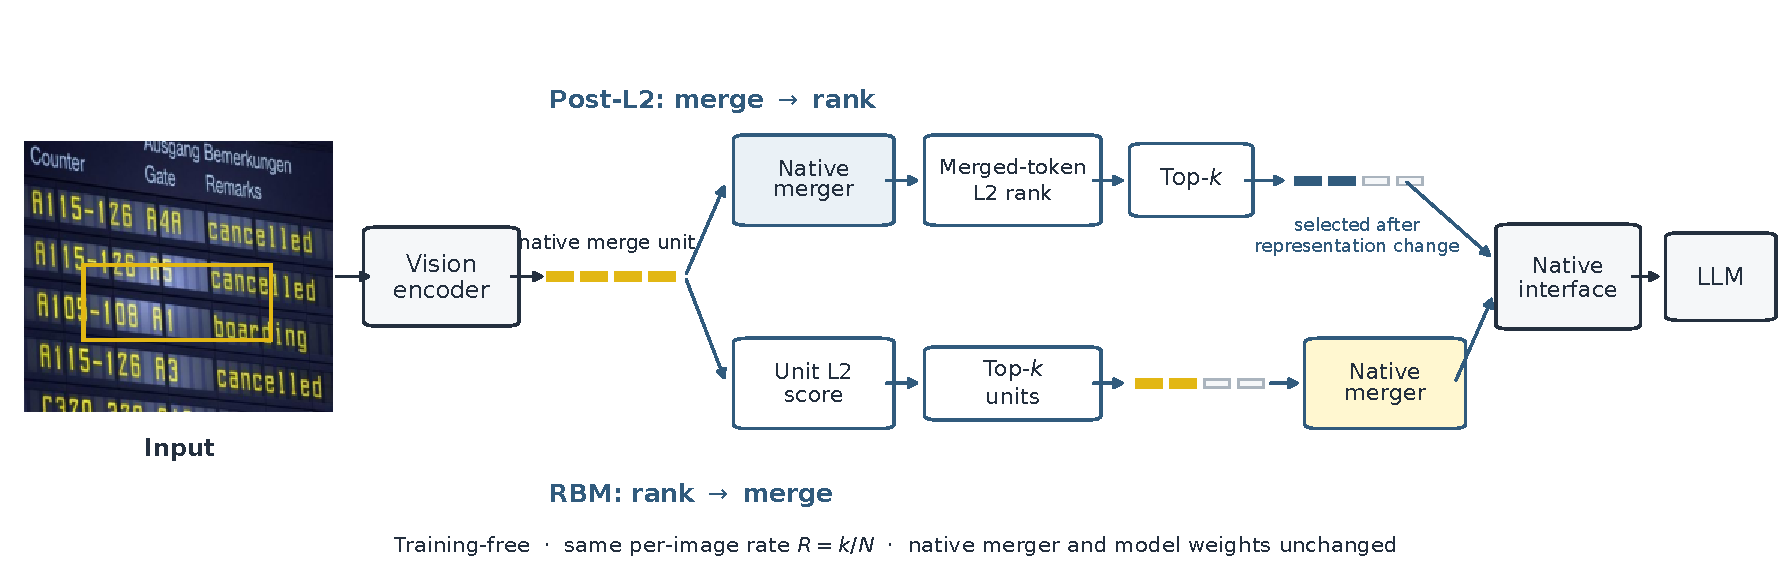
\includegraphics[width=\figurewidth]{figs/fig1_vector.pdf}
  \caption{\label{fig:overview}RBM follows the native merge topology. It ranks
  complete merger-input units, preserves a fixed per-image budget, and passes
  the selected units through the unmodified merger and language-model
  interface. The comparison changes selection order, not model weights.}
\end{figure}

We contribute (1) a formulation that states when representation-dependent
top-$k$ decisions before and after merging agree; (2) RBM, a training-free compressor
with an explicit native-unit and interface contract, validated on three VLMs
and two mergers; (3) RankBridge, a locked probe showing that pre-merger rank
complements FastV attention; and (4) rank, edge-energy, and swap controls that
connect the accuracy gap to merger-induced saliency rewriting.

\Section{Related Work}

Visual-token reduction spans several stages. Methods inside the LLM use
query attention or progressive pruning, including FastV,
PyramidDrop, FasterVLM, and SparseVLM
~\cite{chen2024fastv,xing2024pyramiddrop,zhang2024fastervlm,
zhang2024sparsevlm}. Encoder-output selectors use visual [CLS] attention, graph
propagation, fitted predictors, or multi-cue suppression
~\cite{wang2024vtccls,shang2024prumerge,ye2024fitprune,
jiang2025gprune,luan2025adaptprune}. Unified systems combine saliency with
diversity or text guidance
~\cite{yu2026visiontrim,baek2026agilepruner,fang2026prunesid}.

Merging changes representation as well as length. ToMe uses bipartite matching;
VisionZip preserves dominant tokens and merges the rest; AdaptMerge adds
language guidance
~\cite{bolya2023tome,yang2024visionzip,islam2025adaptmerge}. TokenPacker learns
a compact projector, while GlimpsePrune, VScan, and AnchorPrune target dynamic
or Qwen-family compression
~\cite{li2024tokenpacker,zeng2025glimpseprune,zhang2025vscan,
oh2026anchorprune}. Thus, a selector's input representation is part of the
compression rule.

Recent work broadens selection beyond one attention score. QuietPrune and
PixelPrune move reduction earlier; TransPrune, V2Drop, and Hi-Lo Prune model
token or layerwise variation
~\cite{gao2026quietprune,wang2026pixelprune,li2026transprune,
chen2026v2drop,sun2026hiloprune}. Coverage, reconstruction, and functional
sensitivity guide ApET, SCoRe, CoIn, ZOO-Prune, and SPaRE
~\cite{ma2026apet,xu2026score,du2026coin,kim2026zooprune,lee2026spare}.
Learned or strongly conditioned methods model semantic labels, information
flow, or head importance
~\cite{wang2026metacompress,song2026evocomp,sun2026ifprune,zhu2026hawk}.
Other designs vary token lifetime by layer
~\cite{wang2026informationhorizon,chen2026alvts,li2026crisp}, or preserve
discarded evidence through object-centric, local/global, and hybrid aggregation
~\cite{lei2026core,li2026aot,zhang2026hybrid}. Document-oriented reduction and
provenance audits expose OCR-specific failures
~\cite{choi2026docprune,liu2026provenance}. LMMs-Eval and EffiVLM-Bench provide
the complementary evaluation layer
~\cite{zhang2024lmmseval,wang2025effivlmbench}.

RBM isolates the native-merger boundary. Qwen-VL concatenates four neighboring
patches before LayerNorm and an MLP; InternVL3 uses pixel-shuffle downsampling
~\cite{bai2025qwen3vl,bai2025qwen25vl,zhu2025internvl3}. RBM keeps these
operators and their interface unchanged but ranks their inputs, enabling a
matched pre/post comparison at equal token rate.

\Section{Machine-Centric Compression}

\SubSection{Selection around a native merger}

Let $U=\{u_i\}_{i=1}^{N}$ be the native merge units and let $M$ be the
model's per-unit merger. A representation-dependent scorer produces
$a_i=s_{\mathrm{pre}}(u_i)$ before merging and
$b_i=s_{\mathrm{post}}(M(u_i))$ after merging. At budget $k$, the two decisions
are
\begin{equation}
K_{\mathrm{pre}}=\operatorname{TopK}_{k}\{a_i\},\qquad
K_{\mathrm{post}}=\operatorname{TopK}_{k}\{b_i\}.
\label{eq:sets}
\end{equation}
With deterministic tie breaking, they are equivalent exactly when
$K_{\mathrm{pre}}=K_{\mathrm{post}}$. A sufficient condition for agreement at
every budget is $b_i=g(a_i)$ for a strictly increasing $g$. We measure the
violation at budget $k$ by
\begin{equation}
D_k=1-\frac{|K_{\mathrm{pre}}\cap K_{\mathrm{post}}|}
{|K_{\mathrm{pre}}\cup K_{\mathrm{post}}|}.
\label{eq:disagreement}
\end{equation}
For a fixed set, selection and a per-unit merger are compatible; disagreement
arises when the merger changes the ranking that determines the set.

For compression analysis, define the visual-token rate and task distortion as
\begin{equation}
R=\frac{k}{N},\qquad
\mathcal{D}(R)=1-\frac{S(R)}{S(1)},
\label{eq:rate_distortion}
\end{equation}
where $S(R)$ is the downstream benchmark score at rate $R$. A lower
$\mathcal{D}$ means that more task-relevant information survives. RBM and
Post-L2 have identical $R$, so their vertical separation isolates distortion
introduced by the representation used for selection.

\SubSection{Rank-Before-Merge}

For every image, RBM groups ViT patch features into the model's native
$2\!\times\!2$ units. For a unit $u$ with input patch vectors $h_{u,1:4}$, it
uses the query-blind control score
\begin{equation}
s_{\mathrm{pre}}(u)=\frac{1}{4}\sum_{j=1}^{4}\|h_{u,j}\|_2,
\qquad
s_{\mathrm{post}}(u)=\|M(h_{u,1:4})\|_2.
\end{equation}
It retains $k=\max(1,\operatorname{round}(\kappa N))$ units and applies the
native merger. The contract selects complete units, enforces each image's
exact top-$k$ budget, propagates their identities through main and deepstack
streams, and leaves the merger, positions, interface, and LLM unchanged.
Scoring costs $O(Nd)$ and heap selection $O(N\log k)$. RBM adds no parameters,
question tokens, or LLM-attention pass.

Qwen's merger acts independently per unit, so a fixed kept set produces the
same merged representations; this is byte-identical on the verified Qwen3-VL
path and separates ranking from forward-operator changes.

\SubSection{A merger-aware prior for FastV}

FastV ranks all visual tokens by question-conditioned attention at LLM layer
$K=3$. At $\kappa=0.25$, RankBridge protects
$q=\operatorname{round}(\rho k)$ RBM-ranked positions and fills $k-q$ by FastV
rank. A development gate over $\rho\in\{0.1,0.2,0.3\}$ selected and locked
$\rho=0.2$ for four $n=200$ benchmarks. The endpoints are bit-identical to
FastV ($\rho=0$) and RBM in kept-set identity ($\rho=1$); all candidates remain
available until layer $K$.

\begin{figure}[t]
  \centering
  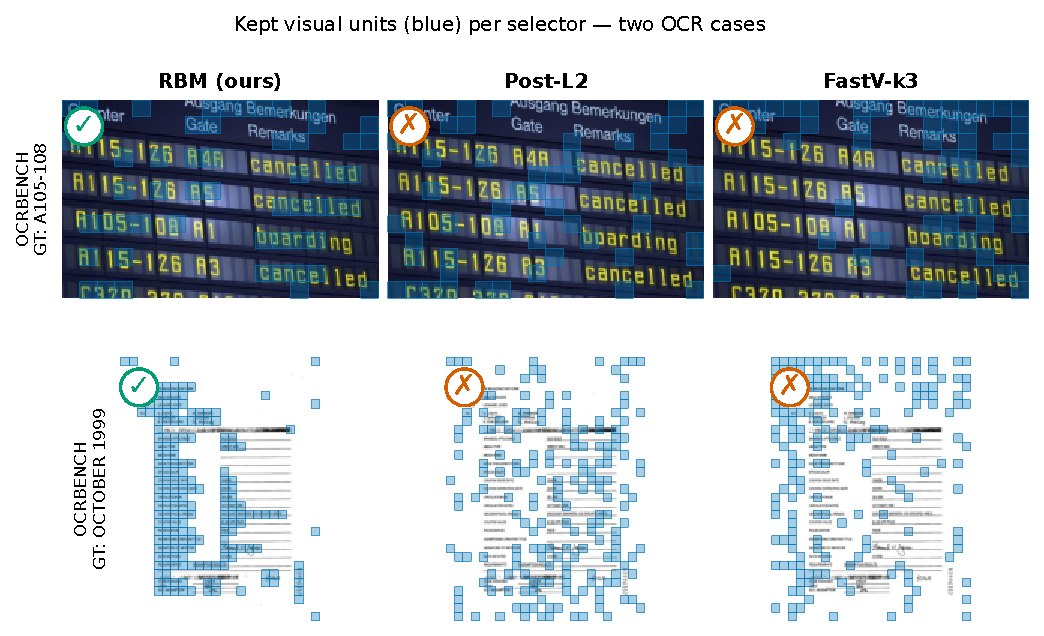
\includegraphics[width=\figurewidth]{figs/fig2_vector.pdf}
  \caption{\label{fig:qualitative}Audited OCRBench examples at 25\% retention.
  RBM, Post-L2, and FastV-k3 preserve different spatial evidence. The examples
  illustrate selection behavior; aggregate results are reported separately.}
\end{figure}

\Section{Experimental Protocol}

We evaluate Qwen3-VL-8B, Qwen2.5-VL-7B, and InternVL3-8B with bf16 weights,
greedy decoding, and family-correct native positions. RBM, uncompressed, and
Post-L2 use vLLM 0.19 V1~\cite{kwon2023vllm}; FastV/RankBridge use HuggingFace
eager attention because FastV lacks a vLLM path. The eager native path matches
8/8 samples, and HF/vLLM uncompressed outputs agree on 16/16 held-out cases.
Throughput is compared only within vLLM.

We use TextVQA VQA accuracy~\cite{singh2019textvqa}, DocVQA
ANLS~\cite{mathew2021docvqa}, OCRBench /1000~\cite{liu2024ocrbench}, and GQA
normalized exact match~\cite{hudson2019gqa}; full splits contain 5000, 5349,
1000, and 12578 items. Scorers port lmms-eval~\cite{zhang2024lmmseval}.
Pre/post tests pair samples and per-image token counts. Nine prespecified
text-dense 25\% comparisons use 20,000 paired-bootstrap resamples and sign-flip
tests with Holm correction (all corrected $p\leq4.5\!\times\!10^{-4}$).
FastV/RankBridge are secondary paired probes on $n=200$.

\Section{Compression Results}

\SubSection{Matched pre- and post-merger selection}

Table~\ref{tab:main} isolates selection stage within query-blind L2 scoring.
At 25\% retention, RBM wins all nine text-dense cells by 11.0--38.4\pp or
235--432 OCRBench points across three VLMs and two merger designs. The gap
widens at 12.5\% on the reported text-dense cells, although RBM remains lossy
relative to no compression.

\begin{table}[t]
\begin{center}
\caption{\label{tab:main}Official full-split results. RBM and Post-L2 use the
same per-image visual-token count. $\Delta$ is RBM minus Post-L2 at 25\%
retention. OCRBench uses points; other rows use percentage points.}
{\renewcommand{\baselinestretch}{0.93}\footnotesize
\setlength{\tabcolsep}{2.5pt}
\begin{tabular}{llrrrr}
\toprule
Model & Benchmark (metric) & None & RBM & Post-L2 & RBM$-$Post \\
\midrule
\multirow{4}{*}{Qwen3-VL}
 & TextVQA (VQA acc.) & .844 & .605 & .222 & $+38.4$ \\
 & DocVQA (ANLS)      & .956 & .481 & .238 & $+24.3$ \\
 & OCRBench (/1000)   & 760  & 547  & 184  & $+363$ \\
 & GQA (EM)           & .616 & .449 & .477 & $-2.8$ \\
\midrule
\multirow{4}{*}{Qwen2.5-VL}
 & TextVQA (VQA acc.) & .862 & .702 & .442 & $+26.1$ \\
 & DocVQA (ANLS)      & .949 & .636 & .526 & $+11.0$ \\
 & OCRBench (/1000)   & 817  & 480  & 182  & $+298$ \\
 & GQA (EM)           & .604 & .559 & .585 & $-2.6$ \\
\midrule
\multirow{4}{*}{InternVL3}
 & TextVQA (VQA acc.) & .8338 & .7890 & .4148 & $+37.4$ \\
 & DocVQA (ANLS)      & .9221 & .7284 & .3820 & $+34.6$ \\
 & OCRBench (/1000)   & 852   & 753   & 321   & $+432$ \\
 & GQA (EM)           & .6293 & .5993 & .6031 & $-0.4$ \\
\bottomrule
\end{tabular}}
\end{center}
\end{table}

GQA marks the boundary: Qwen rankings favor Post-L2 by 2.6--2.8\pp, while
InternVL3's $-0.4$\pp interval crosses zero. A full-split Qwen3-VL control
matched at the merger input still gives RBM $+27.68$\pp TextVQA,
$+4.59$\pp DocVQA, and $+235$ OCRBench, but $-5.64$\pp GQA (95\% CI
$[-6.42,-4.86]$). Selection stage is workload-conditioned.

\SubSection{FastV and the merger-aware prior}

At the same 25\% budget, RankBridge improves FastV-k3 on all four probes
(Table~\ref{tab:rankbridge}). TextVQA gains 3.2\pp ($z=2.11$); the other
0.5--1.6\pp gains are not significant at $n=200$. RBM remains 11.6\pp stronger
on OCRBench, so the hybrid misses its preset within-1\pp gate. Pre-merger rank
adds information to query attention, but one global mixture cannot erase the
workload boundary.

\begin{table}[t]
\begin{center}
\caption{\label{tab:rankbridge}Locked Qwen3-VL probe at 25\% retention
($n=200$). RankBridge protects 20\% of its final budget with the pre-merger
rank and fills the remainder with FastV-k3 attention.}
{\renewcommand{\baselinestretch}{0.95}\small
\setlength{\tabcolsep}{4pt}
\begin{tabular}{lrrrr}
\toprule
Benchmark & RBM & FastV-k3 & RankBridge & RB$-$FastV (pp) \\
\midrule
TextVQA  & .5967 & .7633 & \textbf{.7950} & $+3.2$ \\
DocVQA   & .4239 & .5863 & \textbf{.6023} & $+1.6$ \\
OCRBench & \textbf{.5801} & .4586 & .4641 & $+0.6$ \\
GQA      & .4150 & .5050 & \textbf{.5100} & $+0.5$ \\
\bottomrule
\end{tabular}}
\end{center}
\end{table}

On full OCRBench, RBM exceeds FastV by 14.6\pp on Qwen3-VL and 8.7\pp on
Qwen2.5-VL; FastV is stronger on Qwen3-VL TextVQA/GQA and Qwen2.5-VL TextVQA.
The selectors therefore occupy different regimes.

Figure~\ref{fig:rd} gives rate--distortion operating points: pre-merger
selection lowers text-dense distortion at equal rate, while GQA reverses the
ordering.

\begin{figure}[!b]
  \centering
  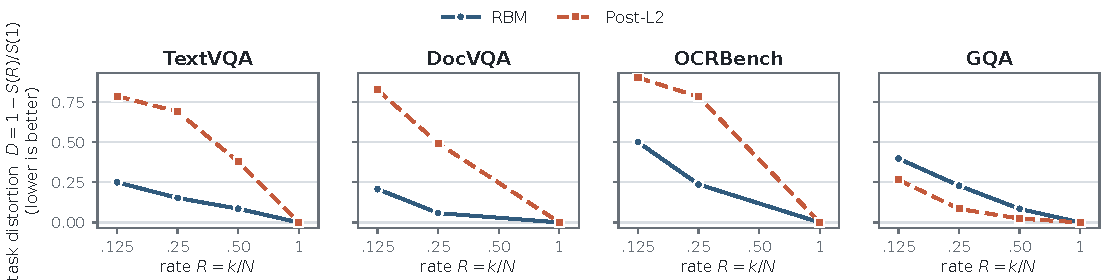
\includegraphics[width=\figurewidth]{figs/fig5_rate_distortion.pdf}
  \caption{\label{fig:rd}Task rate--distortion operating points on the locked
  Qwen3-VL diagnostic subset ($n=200$ per point). Rate is the retained native
  visual-unit fraction; distortion is the relative loss in official task score
  from the uncompressed model. Curves connect measured rates only.}
\end{figure}

\Section{Why the Merger Changes Selection}

Three Qwen3-VL diagnostics explain the gap (Fig.~\ref{fig:mechanism}). Pre/post
ranks correlate weakly: Spearman is 0.137/0.332/0.360 and top-25\% Jaccard is
0.180/0.243/0.278 on DocVQA/TextVQA/GQA. The merger changes the top-$k$ set,
not only score scale.

The change is structured. Correlation between post-minus-pre rank shift and
Sobel edge energy is $+0.439/+0.155/+0.036$. On DocVQA, RBM-only units have
mean edge energy 0.641 versus 0.124 for Post-L2-only units; 92\% versus 35\%
exceed the per-image median. This associates the merger with text-stroke
demotion without attributing it to the training objective.

A ranking-swap control holds the post-merger forward path fixed but uses the
pre-rank. It exactly selects RBM's set (Jaccard $=1.000$), recovers its accuracy,
and yields byte-identical retained outputs. The Qwen3-VL gap therefore comes
from ranking, not a different operation on kept units.

\begin{figure}[!b]
  \centering
  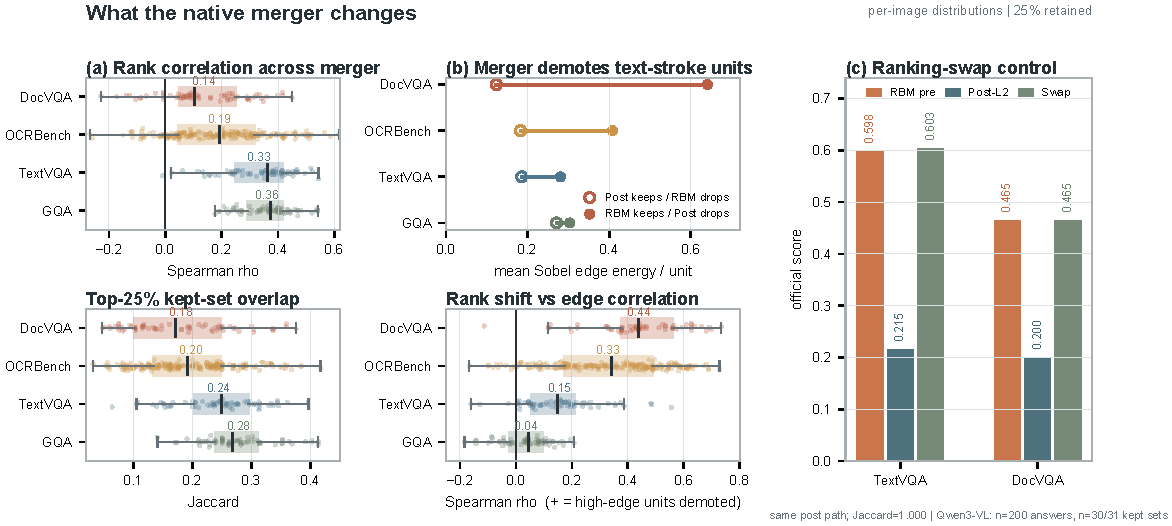
\includegraphics[width=\figurewidth]{figs/fig3_vector.pdf}
  \caption{\label{fig:mechanism}The native merger rewrites selection saliency.
  Rank agreement is low, text-stroke-rich units are demoted, and a ranking-swap
  control restores RBM accuracy with the same kept set.}
\end{figure}

\begin{figure}[t]
  \centering
  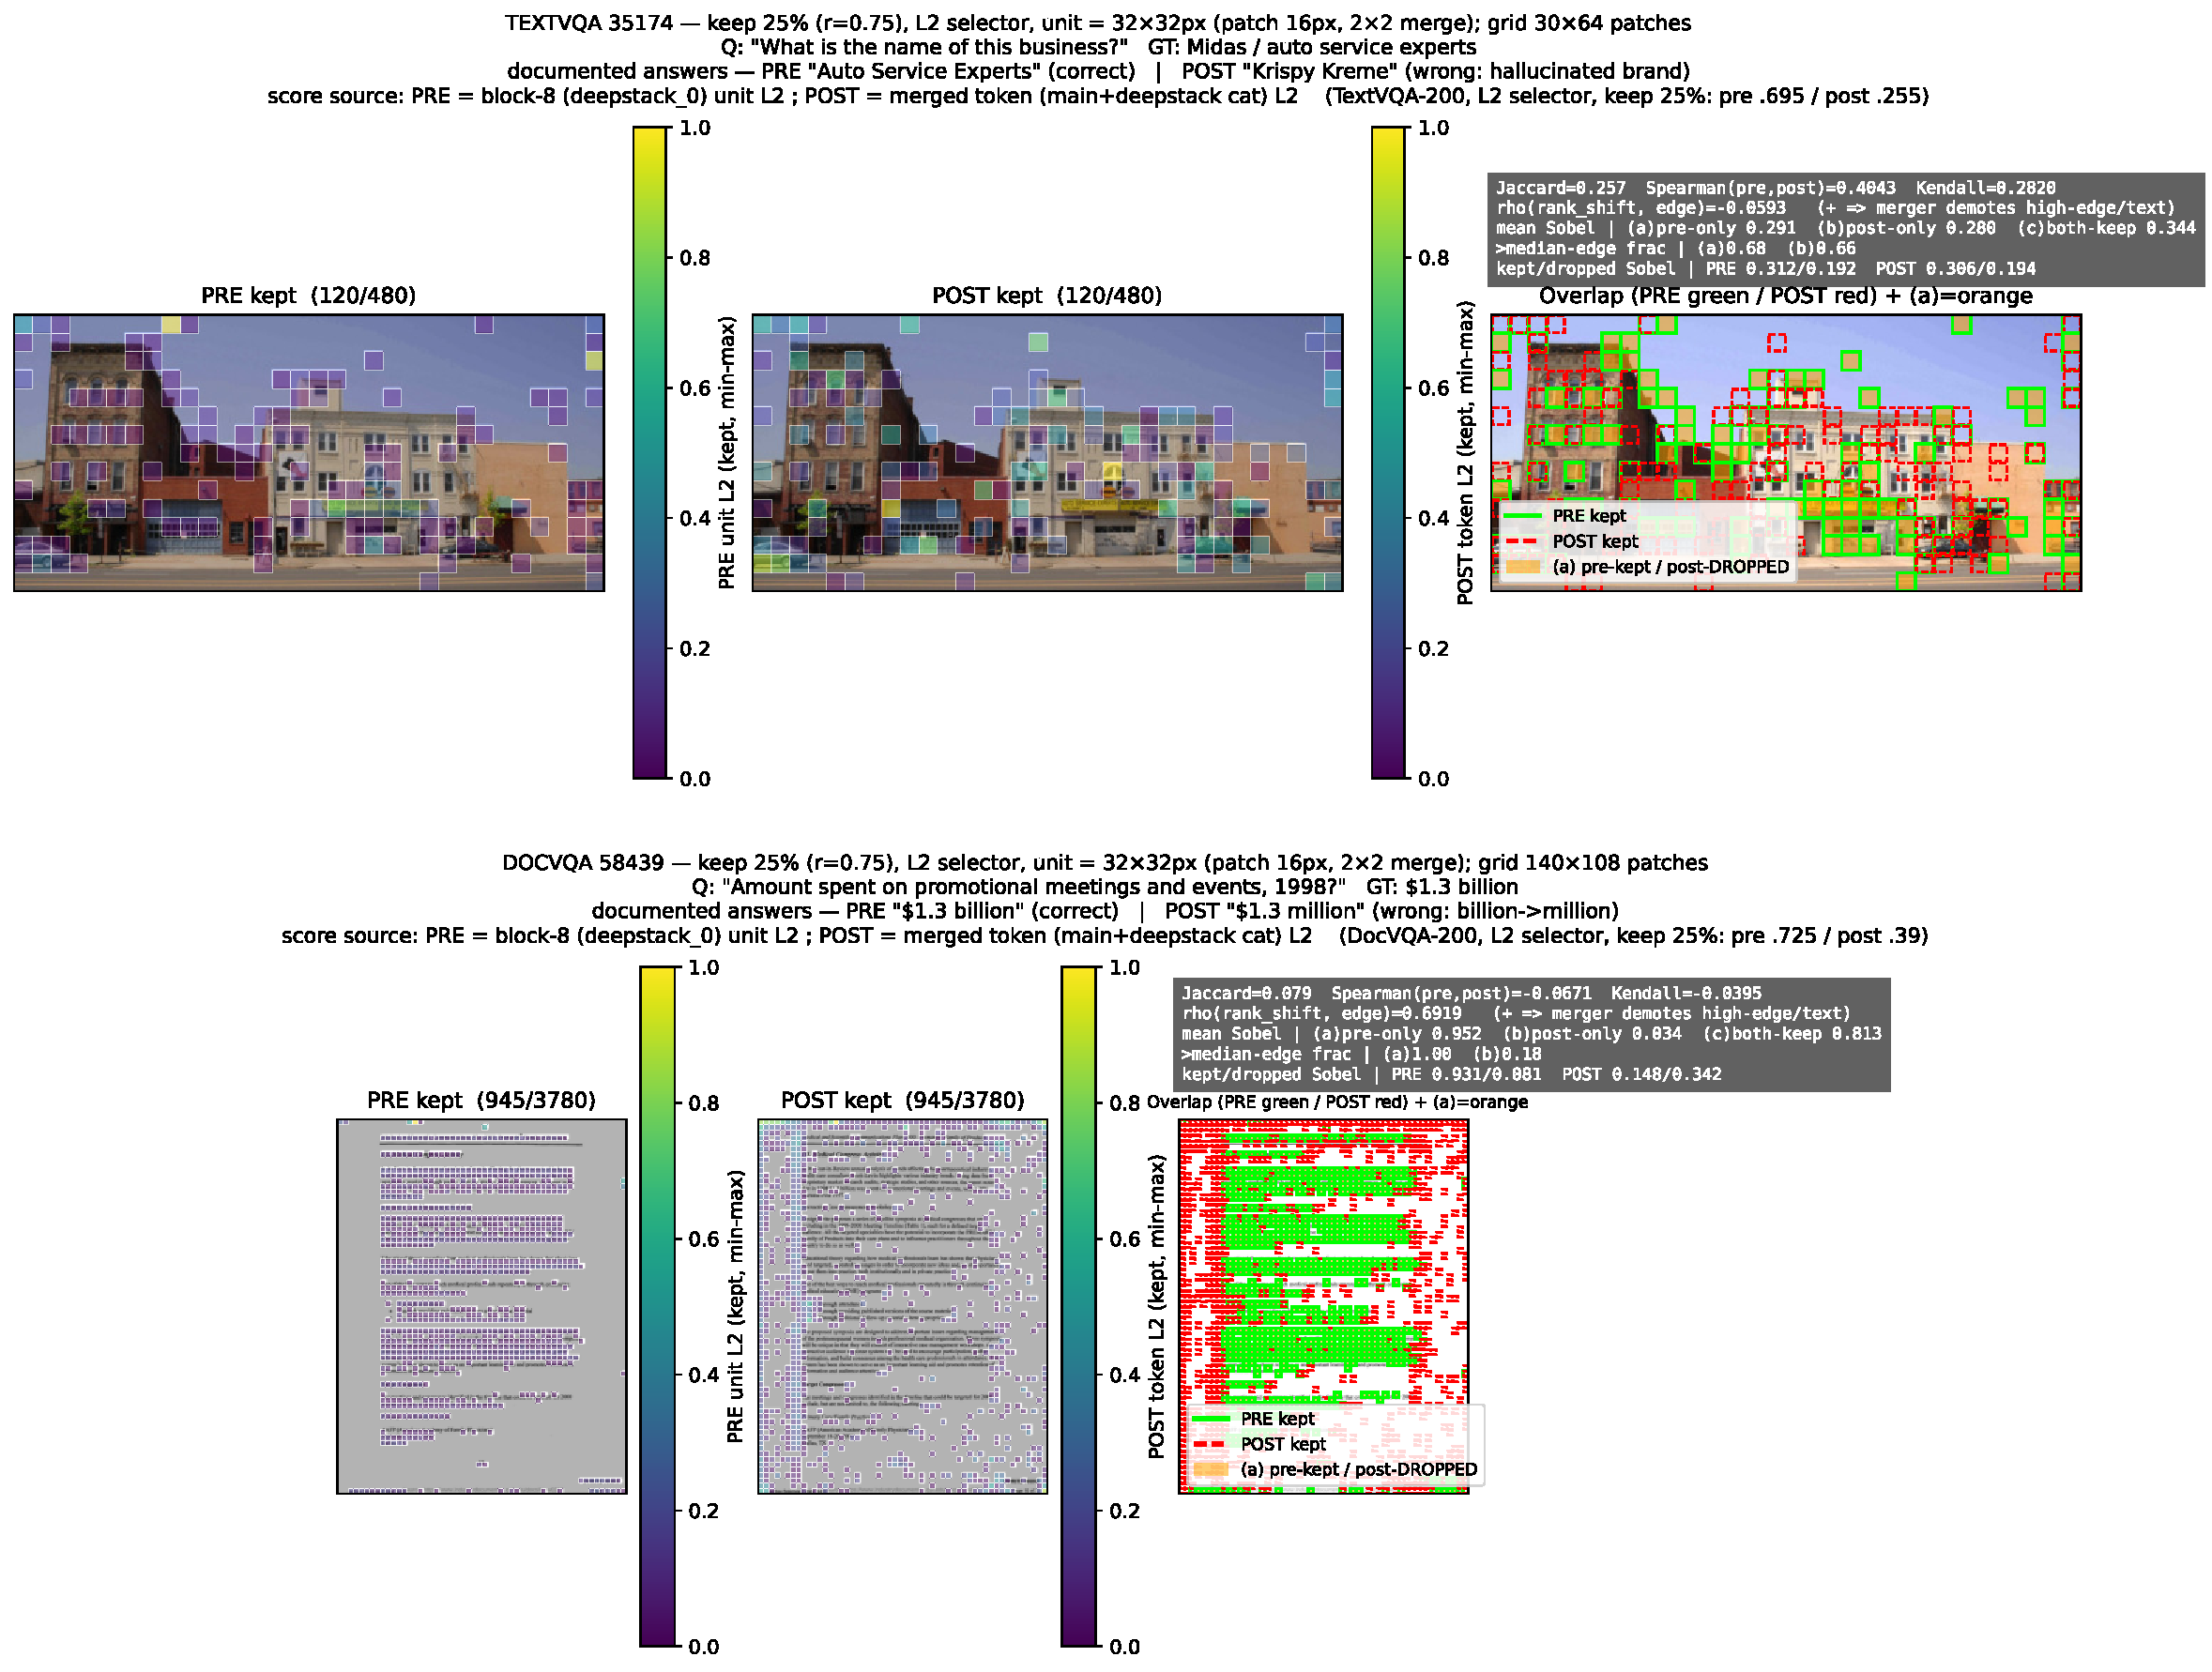
\includegraphics[width=\figurewidth]{figs/fig4_vector.pdf}
  \caption{\label{fig:survival}Token-survival maps for audited TextVQA and
  DocVQA images. Each row shows RBM, Post-L2, and their overlap at the same
  25\% retention. Green and red outlines identify units kept before and after
  merging, respectively. These cases illustrate spatial allocation rather
  than aggregate accuracy.}
\end{figure}

\FloatBarrier

\Section{Efficiency and Scope}

On one A40 with vLLM, RBM versus Post-L2 throughput is 4.61 versus 4.52 at
75\%, 5.39 versus 5.54 at 50\%, and 6.91 versus 6.89 requests/s at 25\%; five
repeats stay within 3\%. RBM gains 12\%, 31\%, and 68\% over no compression;
at 25\%, latency falls from 0.36 to 0.23 seconds. InternVL3 gains
1.8--2.5$\times$. RBM leaves ViT work before its scoring tap intact and
accelerates the merger and LLM sequences.

Byte-exact attribution holds for Qwen3-VL; Qwen2.5-VL retains an ordering
confound, and InternVL3 provides accuracy replication plus a bounded swap.
Models without native merge units are outside scope. FastV/RankBridge use the
eager harness, several secondary cells use $n=200$, and only the TextVQA hybrid
gain is significant. Family pixel caps also preclude absolute cross-model
comparison. The supported claim is merger-aware, text-dense compression, not a
universal selector.

\Section{Conclusion}

Visual-token selection around a native merger is an operator-order problem.
RBM selects complete units at the merger input and applies the unchanged model
to survivors. At equal budgets it preserves more text-dense evidence than
Post-L2 across three VLMs and two mergers while accelerating inference. Its
rank also improves FastV-k3 in four probes, showing complementary signals.
Because the merger rewrites saliency and demotes text-stroke units,
merger-equipped VLM compression should treat topology and selection stage as
first-class constraints.

\Section{References}
\bibliographystyle{IEEEtran}
\bibliography{references}

\end{document}
